\documentclass[12pt,a4paper]{article}
\usepackage[utf8]{inputenc}
\usepackage[german]{babel}
\usepackage[T1]{fontenc}
\usepackage{amsmath}
\usepackage{amsfonts}
\usepackage{amssymb}
\usepackage{graphicx}
\usepackage{siunitx}
\usepackage{float}
\usepackage[left=2cm,right=2cm,top=2cm,bottom=2cm]{geometry}
\usepackage{hyperref}
\author{Gerald}

\begin{document}
\sisetup{separate-uncertainty = true}
	\setlength{\parindent}{0pt} 
	\begin{center}
		{\LARGE Versuchsprotokoll}\\
		\begin{large}
			zum Fortgeschrittenenpraktikum im Bachelorstudiengang Physik\\[0.4cm]
			an der RWTH Aachen\\
			II. Physikalisches Institut A\\[5.5cm]
			\Large\textbf{\textsl{Magnetische Phasenübergänge (PH)}}\\[5.5cm]
			\normalsize\textit{vorgelegt\\von}\\[0.4cm]
			\large{Moritz Berger (355244)\\Gerald Kolter (355005)}\\\textbf{Gruppe 30}\\[2cm]
			\large \textbf{Wintersemester 2017/18}
		\end{large}
	\end{center}
	\newpage
	
	\tableofcontents
	\newpage

\section{Versuchsziel}
Ziel des Versuchs ist es die Sprungtemperatur eines Hochtemperatursupraleiters und die Curie-Temperatur und dadurch die Zusammensetzung einer GdAg$_{1-x}$Zn$_x$-Probe zu bestimmen.

\section{Aufbau}
Der Messaufbau für den Hauptversuch besteht aus einem Hartshorn-Spulensystem, das zusammen mit der darin befindlichen Probe in flüssigem Stickstoff abgekühlt wird. Mit einem Lockin-Verstärker wird die Differenz zwischen den Signalen der beiden gegenläufigen Empfängerspulen gemessen und über ein Multimeter mit dem Messrechner angeschlossen. Unter dem Hartshorn-Spulensystem befindet sich eine Si-Diode zur Messung der Temperatur, die ebenfalls an den Messrechner angeschlossen ist.

\section{Durchführung}
\subsection{Vorversuche}
\subsubsection{Untersuchung eines Tiefpasses}

\begin{figure}
\centering
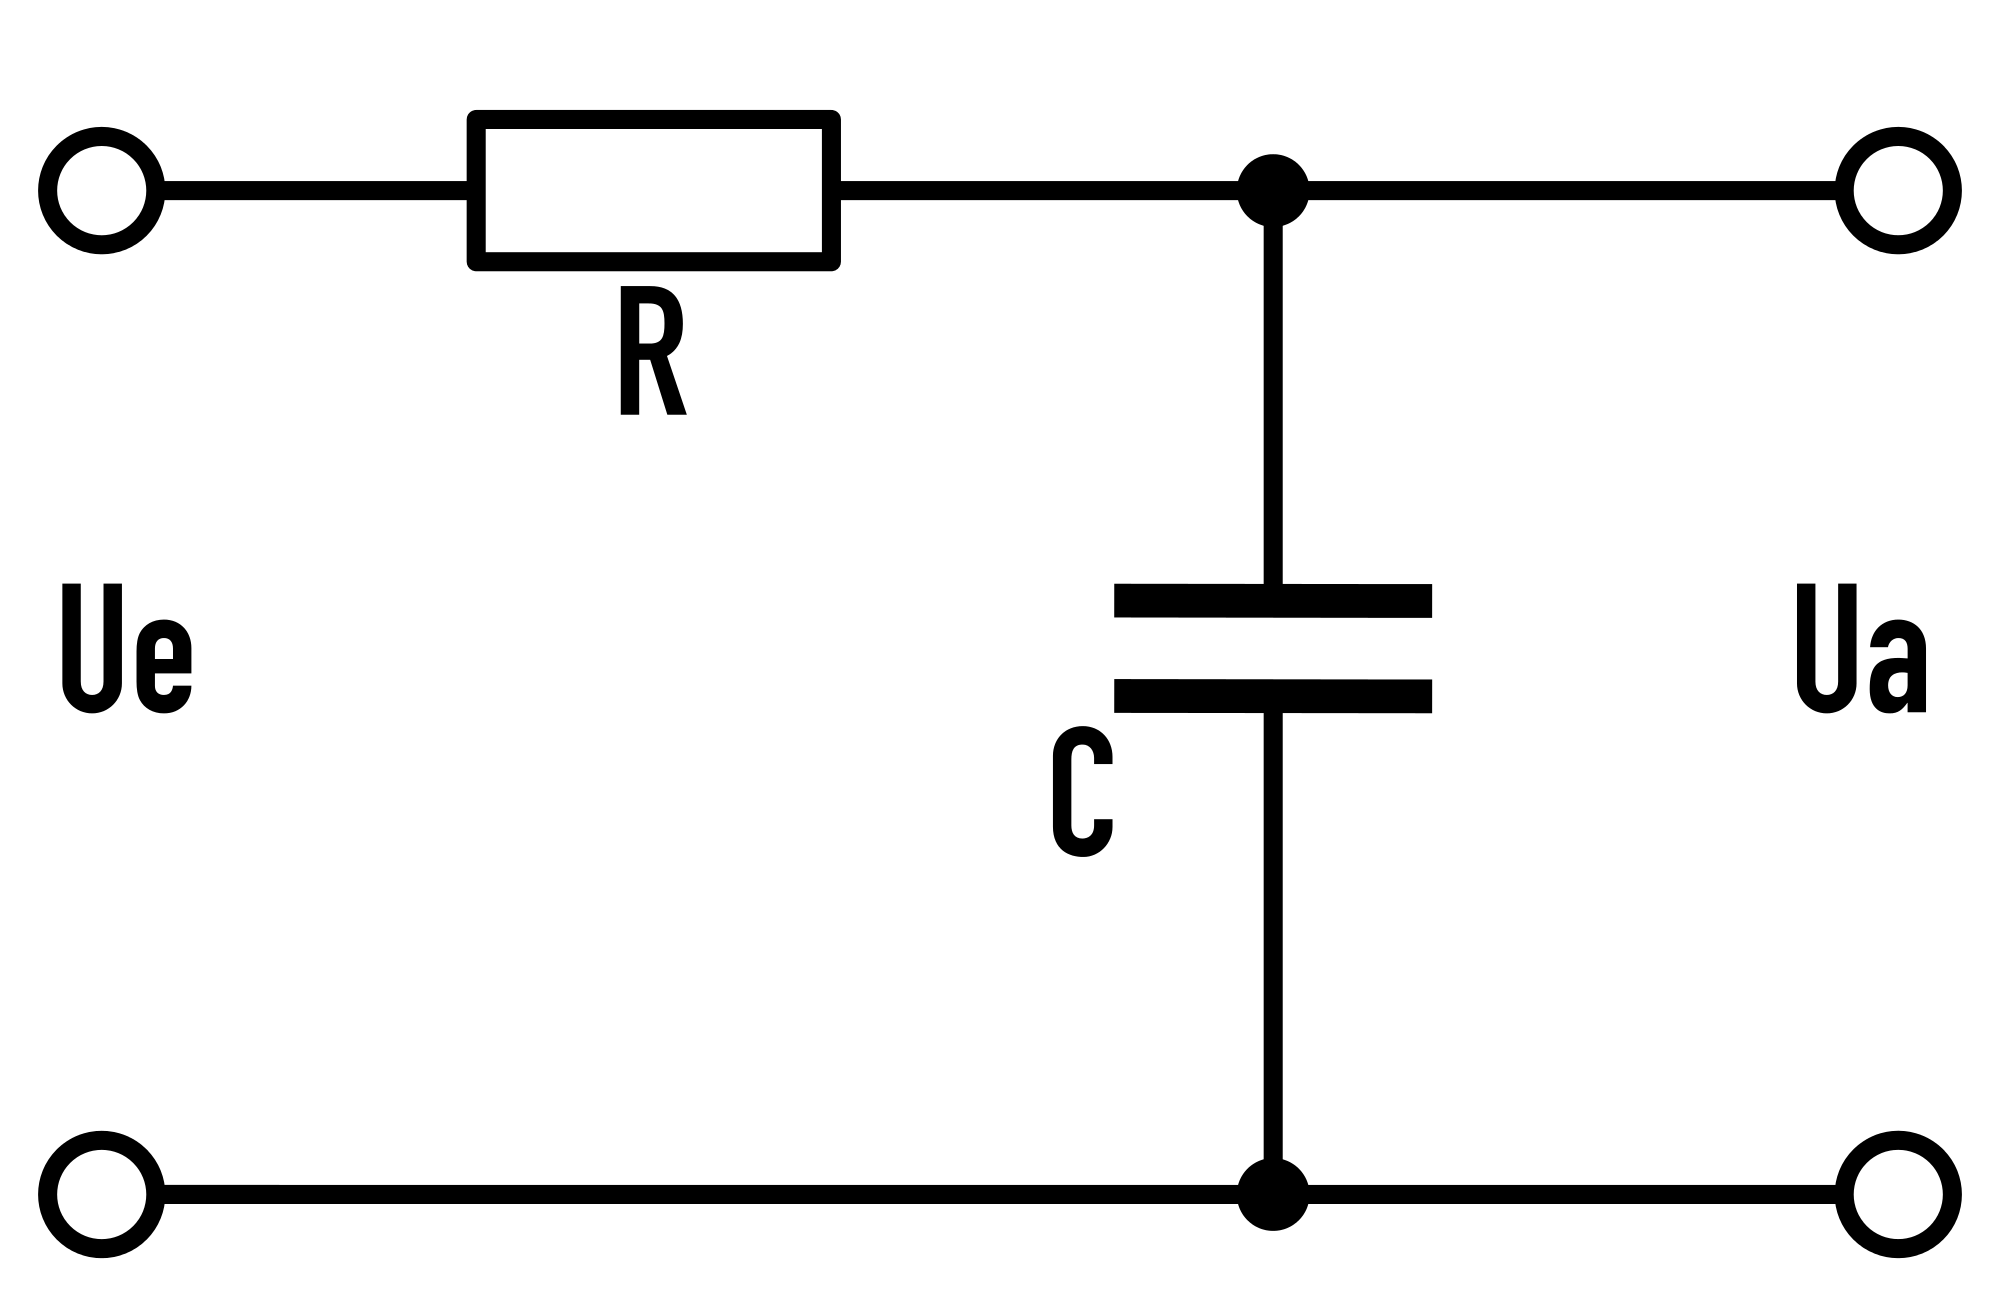
\includegraphics[scale=0.1]{Bilder/Vorversuch1/Tiefpass_Schaltbild.png}
\caption[test]{Schaltbild\footnotemark eines Tiefpasses.}
\label{fig:Tiefpass_Schaltbild}
\end{figure}
%\footnotetext{Quelle: \url{http://de.wikipedia.org/wiki/Tiefpass}}
\footnotetext{Quelle: http://de.wikipedia.org/wiki/Tiefpass}

Mit einem \SI{1,5}{k \Omega} Widerstand und einem \SI{100}{nF} Kondensator wird ein Tiefpass zusammengesetzt. Mit einem Frequenzgenerator wird eine sinusförmige Wechselspannung an den Tiefpass angelegt. Abbildung \ref{fig:Tiefpass_Schaltbild} zeigt das entsprechende Schaltbild. Die angelegte Frequenz wird durchgefahren und dabei werden die an den Tiefpass angelegte und die durch den Tiefpass gefilterte Wechselspannung auf dem Oszilloskop gemessen.

\subsubsection{Untersuchung der Filter des Lockin-Verstärkers}
Das Referenzsignal des Lockin-Verstärkers wird auf einen Eingang des Lockin-Verstärkers gelegt. Die Filterfrequenz wird auf $f_0 = \SI{1000}{Hz}$ eingestellt. Es werden alle drei Filter (Tiefpass-, Hochpass- und Bandpassfilter) des Lockin-Verstärkers vermessen, indem jeweils die Frequenz des Referenzsignals durchgefahren und die Spannungsausgabe des Lockin-Verstärkers gemessen wird.

\subsubsection{Signalfiltern mit Tiefpass und Hochpass}
Mit einem Frequenzgenerator wird eine niedrige Frequenz erzeugt und an einen Eingang des Lockin-Verstärkers gelegt. An den anderen Eingang des Lockin-Verstärkers wird das Referenzsignal des Lockin-Verstärkers gelegt. Mit dem Oszilloskop werden sowohl das Signal des Frequenzgenerators, das Referenzsignal und die Überlagerung der beiden Signale, die der Lockin-Verstärker auf dem SIG.MON Ausgang ausgibt.

\subsubsection{Zeitkonstante und Empfindlichkeit}

\begin{table}
\centering
\begin{tabular}{|c|c|}
\hline 
Integrationszeit $T_I$ & \SI{10}{ms} \\ 
\hline 
Amplitude $U_0$ & \SI{0,5}{V} \\
\hline 
Verstärkung $s$ & \SI{200}{mV} \\ 
\hline 
Phasenschieber & $\varphi = \frac{\pi}{2}$ \\ 
\hline 
\end{tabular} 
\caption{Einstellungen zur Bestimmung einer geeigneten Zeitkonstanten und Empfindlichkeit.}
\label{tab:Zeitkonst_Einstellungen}
\end{table}

Der Lockin-Verstärker integriert das Signal über einen einstellbaren Zeitraum, um so die Schwingung aufgrund der Orthogonalitätsbedingung aus dem Ausgangssignal zu integrieren. \\
Die Empfindlichkeit $s$ des Lockin-Verstärkers wird angegeben in der Spannung, die auf \SI{10}{V} verstärkt wird, sodass sich der Verstärkungsfaktor zu $v = \frac{\SI{10}{V}}{s}$ berechnet. \\
Das Referenzsignal wird auf den Eingang des Lockin-Verstärkers gelegt. Die Frequenz des Referenzsignals wird durchgefahren, um ein geeignetes Verhältnis zwischen Referenzfrequenz und Integrationszeit zu finden. Tabelle \ref{tab:Zeitkonst_Einstellungen} zeigt die verwendeten Einstellungen.


\subsection{Messung des Supraleiters}

\begin{table}
\centering
\begin{tabular}{|c|c|}
\hline 
Integrationszeit $T_I$ & \SI{10}{ms} \\ 
\hline 
Sensitivität $s$ & \SI{500}{\mu V} \\ 
\hline
Filter & Bandpass \\
\hline
Güte & 1 \\
\hline
Filterfrequenz & \SI{380}{Hz} \\
\hline 
Phasenschieber & $\varphi$ = 84.5$^{\circ}$ \\ 
\hline 
Messintervall & \SI{200}{ms} \\ 
\hline 
\end{tabular} 
\caption{Einstellungen für die Messung des Supraleiters.}
\label{tab:Supra_Einstellungen}
\end{table}

Tabelle \ref{tab:Zeitkonst_Einstellungen} zeigt die Einstellungen, die für die Messungen mit dem Supraleiter verwendet wurden. \\
Der Messstab mit dem Supraleiter wird zunächst mit einer Pumpe evakuiert und anschließend mit Helium als Kontaktgas befüllt. Das Ende des Stabes, an dem die Messeinrichtung sitzt, wird zum Kühlen in einen mit flüssigem Stickstoff gefüllten Dewar getaucht und auf ca. \SI{80}{K} gekühlt. Für die Messung wird anschließend der Messstab aus dem Stickstoff herausgezogen, allerdings nur so weit, dass die Erwärmungsrate $\frac{\Delta T}{\Delta t}$ unter \SI{0,1}{K/s} bleibt. Dies ist wichtig, um sicherzustellen, dass zu jedem Zeitpunkt eine möglichst homogene Temperaturverteilung gegeben ist. Während der Erwärmung von \SI{80}{K} auf ca. \SI{120}{K} wird die Temperatur und die Differenzspannung zwischen den beiden Empfängerspulen des Hartshorn-Spulensystems gemessen. \\
Diese Messung wird einmal ohne Probe als Untergrundmessung zur Korrektur und zweimal mit dem Supraleiter durchgeführt: Einmal mit einer Phasenverschiebung zwischen Eingangssignal und Referenzsignal des Lockin-Verstärkers von $\varphi = 0$ und einmal mit einer Phasenverschiebung von $\varphi = \frac{\pi}{2}$, sodass der Realteil ($\varphi = 0$) und der Imaginärteil ($\varphi = \frac{\pi}{2}$) der Suszeptibilität gemessen werden.

\subsection{Messung der Probe}
Bei der Vermessung der GdAg$_{1-x}$Zn$_x$-Probe wird nur der Imaginärteil gemessen. Die Messung wurde ebenfalls bei ca. \SI{80}{K} gestartet, jedoch bis ca. \SI{190}{K} aufgenommen. Aufgrund eines betragsgroßen Offset war der Betrag der an den Lockin-Verstärker angelegten Spannung zu groß, sodass hier die Sensitivität auf \SI{1}{mV} erhöht werden musste.

\section{Ergebnisse}
\subsection{Vorversuche}
\subsubsection{Untersuchung eines Tiefpasses}
Die Messung des Tiefpasses wurde sowohl mit dem Multimeter als auch mit dem Oszilloskop aufgenommen. Dabei wurde mit dem Oszilloskop bei jeder Einstellung der Frequenz ein Bild gemacht, sodass die Auswertung der Oszilloskopdaten auch durch eine Anpassung an Eingangs- und Ausgangssignal geschehen kann. 

\paragraph{Multimeter}
Mit dem Multimeter wird die Effektivspannung von Eingangs- und Ausgangssignal gemessen. Als Fehler auf diese Messungen wird 
\begin{equation*}
\sigma _U = \dfrac{\SI{0,001}{V}}{\sqrt{12}}
\end{equation*}
angenommen. Damit werden der Quotient $\frac{U_a}{U_e}$ und der Fehler durch gaußsche Fehlerfortpflanzung bestimmt. Die zugehörige Frequenz ist die eingestellte Frequenz, auf die der Digitalisierungsfehler
\begin{equation*}
\sigma _f = \dfrac{\SI{1}{Hz}}{\sqrt{12}}
\end{equation*}
angenommen wird. An diese Daten wird eine Anpassung der Form 
\begin{equation}
\dfrac{U_a}{U_e} = \dfrac{1}{\sqrt{1 + \left( \frac{f}{f_G} \right)^2}}
\label{eq:TiefpassFunktion}
\end{equation}
durchgeführt. 

\begin{figure}
\centering
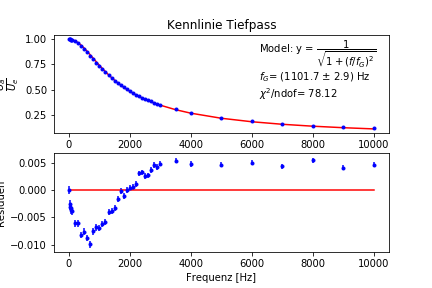
\includegraphics[scale=1]{Bilder/Vorversuch1/TiefpassMulti.png}
\caption[test]{Anpassung der Tiefpassfunktion an die mit dem Multimeter aufgenommenen Daten des selbstgebauten Tiefpasses.}
\label{fig:Tiefpass_Multi}
\end{figure}

Die Anpassung ist in Abbildung \ref{fig:Tiefpass_Multi} gezeigt. Der Verlauf der Daten zeigt, dass das Model durchaus richtig ist. Dennoch zeigen die Residuen gerade bei kleineren Frequenzen eine unbekannte Systematik.

\paragraph{Oszilloskop}
Die Oszilloskopdaten werden mittels Anpassung einer Cosinus-Funktion der Form
\begin{equation*}
U = U_0 \cdot \cos \left( 2 \pi \cdot f  + \varphi _0 \right)
\end{equation*}
ausgewertet. Für diese Anpassungen wird der Fehler auf die gemessene Spannung aus der Differenz der ersten beiden Spannungswerte geteilt durch $\sqrt{12}$ verwendet. Für den Fehler auf die Zeit wird der Abstand zweier Punkte geteilt durch $\sqrt{12}$ verwendet. Die Ergebnisse der Anpassungsparameter und die Fehler darauf sind nur sehr gering abhängig abhängig von den Fehlern, mit denen in diese Anpassung gegangen wird. Da nur die Ergebnisse dieser Parameter und deren Fehler weiter verwendet werden, reicht es, die Fehler für die Cosinus-Anpassung so grob abzuschätzen. \\
Mit den Ergebnissen für die Amplitude und die Frequenzen mit den Fehlern wird erneut eine Tiefpassfunktion (Gl. \ref{eq:TiefpassFunktion}) angepasst.

\begin{figure}
\centering
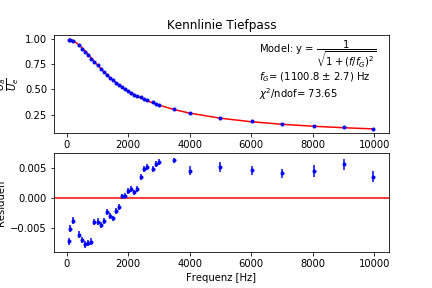
\includegraphics[scale=1]{Bilder/Vorversuch1/TiefpassOszi.png}
\caption[test]{Anpassung der Tiefpassfunktion an die mit dem Oszilloskop aufgenommenen Daten des selbstgebauten Tiefpasses.}
\label{fig:Tiefpass_Oszi}
\end{figure}

Die Anpassung ist in Abbildung \ref{fig:Tiefpass_Oszi} gezeigt. Der Verlauf der Daten zeigt, dass das Model durchaus richtig ist. Dennoch zeigen die Residuen gerade bei kleineren Frequenzen eine unbekannte Systematik. Die Ähnlichkeit zu der Anpassung an die Messung mit dem Multimeter (Abbildung \ref{fig:Tiefpass_Multi}) ist sehr auffällig.

\paragraph{Zusammenfassung}
Betrachtet man die Anpassungen an die mit dem Multimeter (Abbildung \ref{fig:Tiefpass_Multi}) und die mit dem Oszilloskop (Abbildung \ref{fig:Tiefpass_Oszi}) aufgenommenen Daten, fallen zwei Dinge auf:
\begin{enumerate}
\item Die beiden Anpassungen zeigen bei kleineren Frequenzen sehr ähnliche, starke Systematiken, die große $\chi ^2$/ndof bewirken
\item Die Grenzfrequenzen der beiden Anpassungen stimmen innerhalb ihrer Fehler überein
\end{enumerate}
Woher die Systematiken genau kommen ist nicht klar. Da diese aber in beiden Auswertungsmethoden zu sehen sind, ist davon auszugehen, dass sie dem Aufbau entstammen und nicht der Auswertungsmethode. \\
Dass die Grenzfrequenzen innerhalb ihrer Fehler übereinstimmen ermöglicht eine gewichtete Mittelung zu:
\begin{equation*}
f_G = \SI{1101,2 \pm 2,0}{Hz}
\end{equation*}
Die Bauteile des Tiefpasses sind vom Hersteller mit
\begin{equation*}
C = \SI{100 \pm 10}{nF}
\end{equation*}
\begin{equation*}
R = \SI{1500 \pm 15}{\Omega}
\end{equation*}
angegeben. Damit ergibt sich die Grenzfrequenz gemäß
\begin{equation*}
f_G^{Literatur} = \dfrac{1}{2 \pi RC}
\end{equation*}
und der Fehler gemäß
\begin{equation*}
\sigma _{f_G^{Literatur}} = f_G^{Literatur} \cdot \sqrt{\left( \dfrac{\sigma _R}{R} \right) ^2 + \left( \dfrac{\sigma _C}{C} \right) ^2}
\end{equation*}
zu:
\begin{equation*}
f_G^{Literatur} = \SI{1061 \pm 106}{Hz}
\end{equation*}
Der Fehler wird hauptsächlich durch den großen Fehler auf die Kapazität des Kondensators begründet. Damit stimmen Literaturwert und Messergebnis innerhalb ihrer Fehler überein.

\subsubsection{Untersuchung des Tiefpasses des Lockin-Verstärkers}

\begin{figure}
\centering
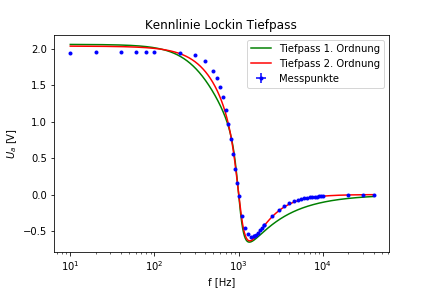
\includegraphics[scale=1]{Bilder/Vorversuch2/KennlinieTiefpass.png}
\caption[test]{Verlauf der Ausgangsspannung bei der Vermessung des Tiefpasses des Lockin-Verstärkers in Abhängigkeit von der Frequenz. In grün und rot sind die Anpassungen der Kennlinien von Tiefpässen 1. und 2. Ordnung.}
\label{fig:LockinTiefpass_Verlauf}
\end{figure}

Bei der Untersuchung der internen Filter wurde nur die Ausgangsspannung gemessen, nicht jedoch die Eingangsspannung. Diese wurde zwar konstant gehalten, um dies jedoch als mögliche Fehlerquelle auszuschließen, wird nur die Ausgangsspannung betrachtet. \\
Den Verlauf der Ausgangsspannung in Abhängigkeit von der Frequenz zeigt Abbildung \ref{fig:LockinTiefpass_Verlauf}. Die Anpassungen der Kennlinien von Tiefpässen 1. bzw. 2. Ordnung sind mit $\chi ^2$/ndof von 2000 bzw. 500 und relativen Fehlern auf die Anpassungsparameter von bis zu $10^4$ nicht gelungen sind. Dennoch zeigen diese, wie in Abbildung \ref{fig:LockinTiefpass_Verlauf} gut erkennbar ist, dass es sich bei dem vermessenen internen Filter des Lockin-Verstärkers um einen Tiefpass 2. Ordnung handelt. \\
Wie bei einem Tiefpass erwartet, werden kleine Frequenzen durchgelassen und hohe Frequenzen unterdrückt. Dazwischen gibt es einen Übergangsbereich von ca. \SI{500}{Hz} bis ca. \SI{1500}{Hz}, in dem das Signal geschwächt durchgelassen wird bzw. teilweise auch mit $(-1)$ multipliziert wird.

\begin{figure}
\centering
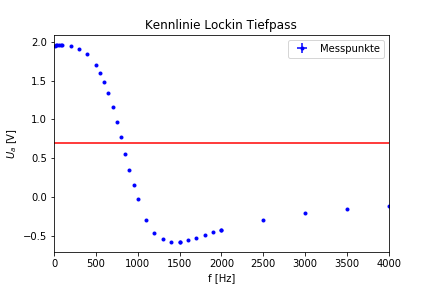
\includegraphics[scale=1]{Bilder/Vorversuch2/AblesenTiefpass.png}
\caption[test]{Verlauf der Ausgangsspannung bei der Vermessung des Tiefpasses des Lockin-Verstärkers in Abhängigkeit von der Frequenz in der Nähe der Grenzfrequenz. In rot ist die horizontale Linie eingezeichnet, bei deren Schnittpunkt mit den Daten die Grenzfrequenz liegt.}
\label{fig:LockinTiefpass_Ablesen}
\end{figure}

Da die Grenzfrequenz nicht aus den Anpassungen bestimmt werden kann, muss diese abgelesen werden. Dazu wird Abbildung \ref{fig:LockinTiefpass_Ablesen} betrachtet, in der die Frequenz zur Vereinfachung des Ablesens nicht logarithmiert und der Frequenzbereich eingeschränkt wurde. Die Grenzfrequenz wird dann abgelesen zu:
\begin{equation*}
f_G^{Tief} = \SI{830 \pm 14}{Hz}
\end{equation*}
Der Fehler wird dabei aus der Annahme einer Gleichverteilung zwischen den beiden Messpunkten um den Schnittpunkt abgeschätzt.

\subsubsection{Untersuchung des Hochpasses des Lockin-Verstärkers}

\begin{figure}
\centering
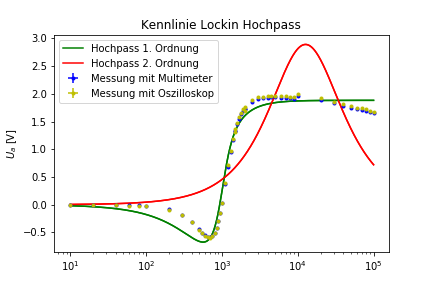
\includegraphics[scale=1]{Bilder/Vorversuch2/KennlinieHochpass.png}
\caption[test]{Verlauf der Ausgangsspannung bei der Vermessung des Hochpasses des Lockin-Verstärkers in Abhängigkeit von der Frequenz. In grün und rot sind die Anpassungen der Kennlinien von Hochpässen 1. und 2. Ordnung.}
\label{fig:LockinHochpass_Verlauf}
\end{figure}

Auch beim Hochpass wurde die Eingangsspannung nicht aufgenommen und deshalb nur die Ausgangsspannung betrachtet. \\
Auch hier sind die Anpassungen nicht gelungen. Dennoch zeigt Abbildung \ref{fig:LockinHochpass_Verlauf}, dass es sich bei dem vermessenen Hochpass des Lockin-Verstärkers um einen Hochpass 1. Ordnung handelt, da diese Anpassung die Daten deutlich besser beschreibt als die eines Hochpasses 2. Ordnung. \\
Wie bei einem Hochpass erwartet, werden kleine Frequenzen unterdrückt und hohe Frequenzen durchgelassen. Dazwischen gibt es wieder einen Übergangsbereich, wobei dieser bereits bei kleineren Frequenzen beginnt, nämlich bei ca. \SI{150}{Hz} und auch etwas weiter geht, bis ca. \SI{2}{kHz}. Abgesehen davon sieht der Übergangsbereich qualitativ dem Übergangsbereich des Tiefpasses ähnlich nur umgedreht.

\begin{figure}
\centering
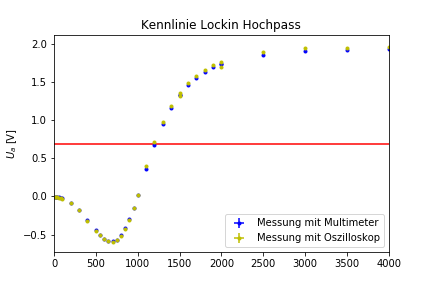
\includegraphics[scale=1]{Bilder/Vorversuch2/AblesenHochpass.png}
\caption[test]{Verlauf der Ausgangsspannung bei der Vermessung des Hochpasses des Lockin-Verstärkers in Abhängigkeit von der Frequenz in der Nähe der Grenzfrequenz. In rot ist die horizontale Linie eingezeichnet, bei deren Schnittpunkt mit den Daten die Grenzfrequenz liegt.}
\label{fig:LockinHochpass_Ablesen}
\end{figure}

Auch hier wird die Grenzfrequenz durch Ablesen bestimmt. Dazu ist in Abbildung \ref{fig:LockinHochpass_Ablesen} der Bereich um die Grenzfrequenz in nicht-logarithmischer Auftragung gezeigt. Die Grenzfrequenz wird dann abgelesen zu:
\begin{equation*}
f_G^{Hoch} = \SI{1200 \pm 29}{Hz}
\end{equation*}
Der Fehler wird dabei wieder aus der Annahme einer Gleichverteilung zwischen den beiden Messpunkten um den Schnittpunkt abgeschätzt.

\subsubsection{Untersuchung des Bandpasses des Lockin-Verstärkers}

\begin{figure}
\centering
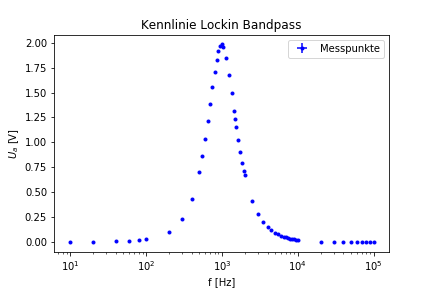
\includegraphics[scale=1]{Bilder/Vorversuch2/KennlinieBandpass.png}
\caption[test]{Verlauf der Ausgangsspannung bei der Vermessung des Bandpasses des Lockin-Verstärkers in Abhängigkeit von der Frequenz.}
\label{fig:LockinBandpass_Verlauf}
\end{figure}

Auch beim Bandpass wurde die Eingangsspannung nicht aufgenommen und deshalb nur die Ausgangsspannung betrachtet. \\
Hier wurden Anpassungen durchgeführt, da der Bandpass sehr wahrscheinlich durch Kombination der bereits vermessenen Tief- und Hochpass zusammengesetzt ist. \\
Abbildung \ref{fig:LockinBandpass_Verlauf} zeigt den gemessenen Verlauf der Ausgangsspannung in Abhängigkeit von der Frequenz. Wie bei einem Bandpass erwartet werden sowohl hohe als auch niedrige Frequenzen unterdrückt. In einem Bereich von ca. \SI{300}{Hz} bis ca. \SI{5}{kHz} werden die Frequenzen durchgelassen, wobei die Durchlassfunktion eine Gaußglockform hat.

\begin{figure}
\centering
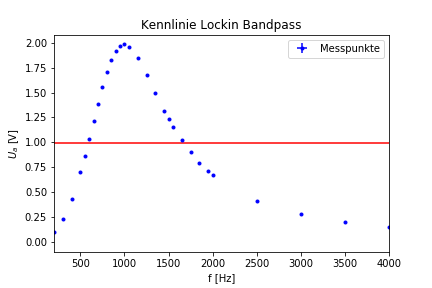
\includegraphics[scale=1]{Bilder/Vorversuch2/AblesenBandpass.png}
\caption[test]{Verlauf der Ausgangsspannung bei der Vermessung des Bandpasses des Lockin-Verstärkers in Abhängigkeit von der Frequenz in der Nähe der Grenzfrequenz. In rot ist die horizontale Linie eingezeichnet, bei deren Schnittpunkten die beiden den Peak begrenzenden Frequenzen liegen.}
\label{fig:LockinBandpass_Ablesen}
\end{figure}

Für die Bestimmung der Güte des Bandpasses werden die beiden den Peak begrenzenden Frequenzen $f_H$ und $f_L$ abgelesen. Mit diesen kann gemäß
\begin{equation*}
f_G = \sqrt{f_H \cdot f_L}
\end{equation*}
die Grenzfrequenz und mit
\begin{equation*}
Q = \dfrac{f_G}{f_H - f_L}
\end{equation*}
die Güte bestimmt werden. Die Fehler bestimmen sich nach gaußscher Fehlerfortpflanzung durch:
\begin{equation*}
\sigma _{f_G} = \sqrt{\left( \dfrac{\sigma _{f_H} \cdot f_H}{2 \cdot f_G} \right)^2 + \left( \dfrac{\sigma _{f_L} \cdot f_L}{2 \cdot f_G} \right)^2}
\end{equation*}
Die begrenzenden Frequenzen werden abgelesen zu:
\begin{equation*}
f_L = \SI{600 \pm 14}{Hz}
\end{equation*}
\begin{equation*}
f_H = \SI{1650 \pm 14}{Hz}
\end{equation*}
Der Fehler wird dabei wieder aus der Annahme einer Gleichverteilung zwischen den beiden Messpunkten um den Schnittpunkt abgeschätzt. \\
Damit bestimmen sich die Grenzfrequenz und die Güte zu:
\begin{equation*}
f_G = \SI{994 \pm 12}{Hz}
\end{equation*}
\begin{equation*}
Q = 0,948 \pm 0,021
\end{equation*}

\subsubsection{Zusammenfassung interne Filter des Lockin-Verstärkers}
Die Filter hatten alle qualitativ den erwarteten Verlauf in ihrer Übertragungsfunktion. Die Ergebnisse für die Grenzfrequenzen von Hoch- und Tiefpass liegen allerdings deutlich neben der eingestellten Frequenz von \SI{1000}{Hz}. Die Ursache davon ist unbekannt. \\
Dennoch stimmt die Grenzfrequenz des Bandpasses innerhalb ihres Fehlers mit der Erwartung von erneut \SI{1000}{Hz} überein. Der Messwert für die Güte liegt ca. 2,45$\sigma$ neben dem eingestellten Wert von 1. Da in den weiteren Messungen der Bandpass verwendet wurde, kann davon ausgegangen werden, dass der Lockin-Verstärker wie erwünscht funktioniert.

\subsubsection{Signalfiltern mit Tiefpass und Hochpass}
\subsubsection{Zeitkonstante und Empfindlichkeit}
\subsection{Messung des Supraleiters}
\subsection{Messung der Probe}

\begin{figure}
\centering
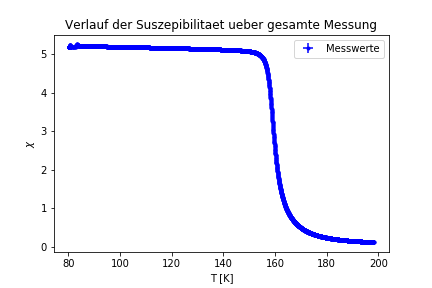
\includegraphics[scale=1]{Bilder/Haupt_Probe/Suszeptibilitaet_Verlauf.png}
\caption[test]{Verlauf der Suszeptibilität über die gesamte Messung.}
\label{fig:Suszeptibilitaet_Verlauf}
\end{figure}

Für die Messung der Probe wurde eine Phase von \SI{180}{\degree} verwendet, daher sind die Daten an der X-Achse gespiegelt. Zudem ist ein sehr großer Offset in den Daten, der noch zu bestimmen ist. \\
Für die Umrechnung der in der Messung aufgenommenen Spannung nach Korrektur des Offset in Suszeptibilität gilt folgender Zusammenhang:
\begin{equation*}
\chi = \dfrac{U}{C \cdot v \cdot V_{Probe} \cdot (1-n_M)}
\end{equation*}
Dabei sind
\begin{equation*}
C = 8034,7 \, \pm \, 34,7
\end{equation*}
die mit dem Supraleiter bestimmte Kalibrationskonstante, 
\begin{equation*}
V_{Probe} = \SI{22,90 \pm 0,05}{mm^3}
\end{equation*}
das Probenvolumen,
\begin{equation*}
n_M = 0,27
\end{equation*}
der Entmagnetisierungsfaktor und 
\begin{equation*}
v = \dfrac{\SI{10}{V}}{s}
\end{equation*}
der Verstärkungsfaktor, wobei $s$ die Sensitivität ist, die in diesem Versuch auf \SI{1}{mV} gestellt werden musste, da der Lockin-Verstärker ansonsten in einen Overload gelaufen wäre. Abbildung \ref{fig:Suszeptibilitaet_Verlauf} zeigt den Verlauf der Suszeptibilität der Probe über die gesamte Messung. 

\subsubsection{Curie-Weiss-Gesetz}
Für einen Temperaturbereich deutlich oberhalb der Grenztemperatur $T_C$ gilt der Zusammenhang:
\begin{equation*}
\chi ^{-1} = \dfrac{T - T_C}{C_{Curie}}
\end{equation*}
Dabei ist $C_{Curie}$ die materialabhängige Curie-Konstante. Daher ergibt sich bei Auftragung von $\chi ^{-1}$ gegen T ein linearer Zusammenhang. In Abbildung \ref{fig:Suszeptibilitaet_Verlauf} ist zu erkennen, dass die Grenztemperatur bei ca. \SI{160}{K} liegt, sodass der Bereich für diese Anpassung gewählt wird zu \SI{180}{K} - \SI{190}{K}. \\
Mit dieser Anpassung wird der Offset gewählt. Dazu wird die Anpassung für verschiedene Offsets in einem Bereich von \SI{0}{V} bis \SI{1,8}{V} in 10000 äquidistanten Schritten durchgeführt und derjenige Offset verwendet, der in der Anpassung das niedrigste $\chi ^2$/ndof ergeben hat. Dieses liegt mit 0.34 zu niedrig, es wurden also vermutlich die Fehler überschätzt.

\begin{figure}
\centering
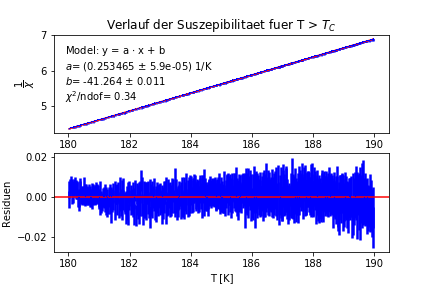
\includegraphics[scale=1]{Bilder/Haupt_Probe/CurieWeiss.png}
\caption[test]{Lineare Anpassung bei Auftragung von $\chi ^{-1}$ gegen T in einem Bereich von \SI{180}{K} - \SI{190}{K}.}
\label{fig:CurieWeiss}
\end{figure}

Abbildung \ref{fig:CurieWeiss} zeigt die lineare Anpassung bei dem bestimmten Offset. Die Grenztemperatur berechnet sich aus den Anpassungsparametern zu:
\begin{equation}
T_C = -\dfrac{b}{a}
\label{eq:ProbeGrenztemperatur}
\end{equation}
Die Fehler auf die Parameter pflanzen sich fort zu:
\begin{equation}
\dfrac{\sigma _{T_C}}{T_C} = \sqrt{\left( \dfrac{\sigma _a}{a} \right)^2 + \left( \dfrac{\sigma _b}{b} \right)^2}
\label{eq:ProbeGrenztemperaturFehler}
\end{equation}
Der Wert für die Grenztemperatur ergibt sich zu (systematische Fehler werden später betrachtet):
\begin{equation*}
T_C^{(1)} = \SI{162,800 \pm 0,057}{K}
\end{equation*}

\subsubsection{Temperaturen nahe der Grenztemperatur}

\begin{figure}
\centering
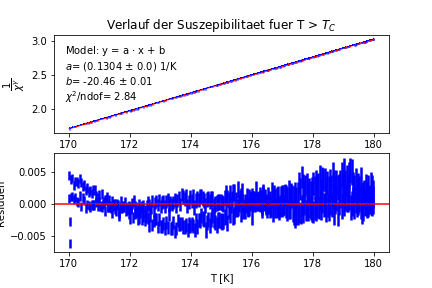
\includegraphics[scale=1]{Bilder/Haupt_Probe/CurieWeiss_gamma.png}
\caption[test]{Lineare Anpassung bei Auftragung von $\chi ^{\frac{-1}{\gamma}}$ gegen T in einem Bereich von \SI{170}{K} - \SI{180}{K}.}
\label{fig:CurieWeiss_gamma}
\end{figure}

In einem Bereich nah an der Grenztemperatur wird der Zusammenhang besser beschrieben durch:
\begin{equation*}
\chi ^{-1} \propto (T - T_C)^\gamma
\end{equation*}
Wobei für den kritischen Exponenten des Phasenübergangs $\gamma \approx \dfrac{4}{3}$ gilt. \\
Es wird der Offset verwendet, der sich bei der ersten Anpassung als der beste herausgestellt hat. \\
Bei Auftragung von $\chi ^{\frac{-1}{\gamma}}$ gegen T ergibt sich erneut ein linearer Zusammenhang, an den ebenfalls eine Anpassung durchgeführt wird. Der Bereich für diese Anpassung wurde gewählt zu \SI{170}{K} - \SI{180}{K}. Diese Anpassung ist in Abbildung \ref{fig:CurieWeiss_gamma} dargestellt. Die Anpassung kann bei einem $\chi ^2$/ndof von 2.84 als gelungen betrachtet werden. Die Grenztemperatur und der Fehler bestimmen sich gemäß Gl. \ref{eq:ProbeGrenztemperatur} und Gl. \ref{eq:ProbeGrenztemperaturFehler} zu:
\begin{equation*}
T_C^{(2)} = \SI{156,862 \pm 0,061}{K}
\end{equation*}

\subsubsection{Temperaturgradient}

\begin{figure}
\centering
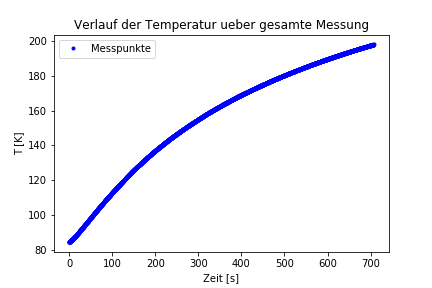
\includegraphics[scale=1]{Bilder/Haupt_Probe/Temperatur_Verlauf.png}
\caption[test]{Temperaturverlauf bei der Messung der Probe.}
\label{fig:TemperaturverlaufProbe}
\end{figure}

\begin{figure}
\centering
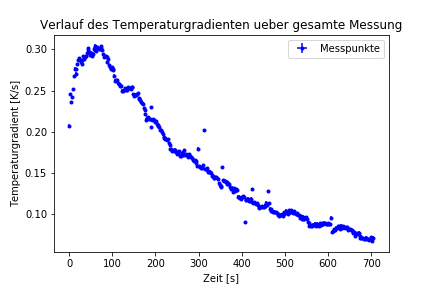
\includegraphics[scale=1]{Bilder/Haupt_Probe/Temperaturgradient_Verlauf.png}
\caption[test]{Verlauf des Temperaturgradienten bei der Messung der Probe.}
\label{fig:TemperaturgradientverlaufProbe}
\end{figure}

Bei der Messung wird in Intervallen \SI{200}{ms} u.a. die Temperatur gemessen. Damit ergibt sich der in Abbildung \ref{fig:TemperaturverlaufProbe} gezeigte Temperaturverlauf. \\
Den Temperaturgradienten erhält man nun aus der Ableitung des Temperaturverlaufs. Da die Datenpunkte deutlich schwanken, wird diese Ableitung bestimmt, indem immer an 20 Punkte eine lineare Regression durchgeführt wird. Der Mittelwert der Zeiten der 20 Temperaturpunkte und die Steigung ergeben dann Punktepaare des Temperaturgradienten. Der Verlauf des Temperaturgradienten ist in Abbildung \ref{fig:TemperaturgradientverlaufProbe} dargestellt. Daran ist deutlich zu sehen, dass der Temperaturgradient bei der Messung der Probe bis zu einer Temperatur von ca. \SI{180}{K} oberhalb der ursprünglich gesetzten Grenze von \SI{0,1}{K/s} liegt.

\subsubsection{Systematischer Fehler}
Die statistischen Fehler auf die aus den beiden Methoden bestimmten Grenztemperaturen sind sehr klein gegen die Differenz der beiden. Daher ist eine Betrachtung der Systematiken sehr wichtig. \\
Fehlerquelle, die als systematisch betrachtet werden kann, sind die Fehler auf die Werte, die zur Umrechnung von der Spannung auf die Suszeptibilität verwendet werden. Die Fehler pflanzen sich fort durch: 
\begin{equation*}
\dfrac{\sigma _{\chi}}{\chi} = \sqrt{\left( \dfrac{\sigma _C}{C} \right)^2 + \left( \dfrac{\sigma _v}{v} \right)^2 + \left( \dfrac{\sigma _V}{V} \right)^2 + \left( \dfrac{\sigma _{n_M}}{1 - n_M} \right)^2}
\end{equation*}
Dabei entstammt der Fehler auf die Kalibrationskonstante der Bestimmung derselben. Der Fehler auf das Probenvolumen bestimmt sich durch gaußsche Fehlerfortpflanzung aus den Ablesefehlern auf die mit einer Schieblehre gemessenen Dimensionen der Probe. Auf den Entmagnetisierungfaktor wird der Digitalisierungsfehler angenommen und auf den Verstärkungsfaktor ein Fehler von 5\% angenommen. Nun wird die Suszeptibilität um diesen Fehler in beide Richtungen verschoben und die Anpassungen erneut durchgeführt. Aus der Veränderung des Ergebnisses für die Grenztemperatur ergibt sich der systematische Fehler aus den Fehlern auf Kalibrationskonstante, Probenvolumen, Verstärkungsfaktor und Entmagnetisierungsfaktor, sodass sich insgesamt für die Grenztemperaturen die folgenden Werte ergeben:
\begin{equation*}
T_C^{(1)} = (162,800 \pm 0,057 \; (stat.) \; \; ^{+0,0000090}_{-0,0000086} \; (sys.)) \, \si{K}
\end{equation*}
\begin{equation*}
T_C^{(2)} = (156,8623 \pm 0,0615 \; (stat.) \; \; ^{+5,9370}_{-0,0030} \; (sys.)) \, \si{K}
\end{equation*}
Drei der vier Fehler (vier Fehler durch die Asymmetrie) sind eine Größenordnung oder mehr kleiner als die statistischen Fehler. Der vierte Fehler ist zwei Größenordnungen größer als der statistische Fehler und sorgt dafür, dass die beiden Werte für die Grenztemperatur innerhalb ihrer Fehler übereinstimmen. Woher der große Unterschied der systematischen Fehler kommt, ist unklar. \\
Dazu kommt noch ein Fehler durch den zu hohen Temperaturgradienten während der Messung. Den Betrag dieses Fehlers abzuschätzen ist schwierig. Da sich allerdings die Si-Diode, die zur Messung der Temperatur verwendet wird, unter dem Hartshorn-Spulensystem befindet, ist die gemessene Temperatur bei zu großem Temperaturgradient kleiner als die Temperatur der Probe. Dies liegt daran, dass der Probenstab nicht vollständig aus dem Dewar gezogen wird, sodass die Kühlung, die das Aufwärmen verlangsamt, die Diode und das Spulensystem von unten kühlt. Da der Temperaturgradient in dem Bereich, in dem die Anpassung für $T_C^{(1)}$ durchgeführt wurde, kleiner ist, als der Bereich, in dem die Anpassung für $T_C^{(2)}$ durchgeführt wurde, ist davon auszugehen, dass dieser Effekt die beiden Werte ''zusammenschieben''  würde.

\subsubsection{Zusammenfassung}

\begin{figure}
\centering
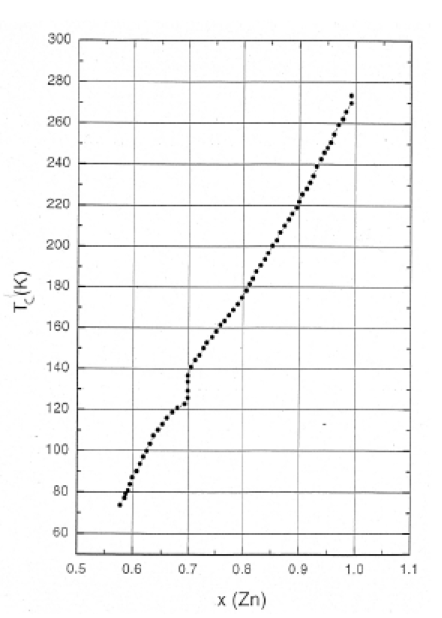
\includegraphics[scale=1]{Bilder/Haupt_Probe/Anteilbestimmung.png}
\caption[test]{Zusammensetzung der Probe in Abhängigkeit der Grenztemperatur\footnotemark.}
\label{fig:AnteilbestimmungProbe}
\end{figure}
\footnotetext{Quelle: Versuchsanleitung Seite 32.}

Die beiden Anpassungsbereiche haben Grenztemperaturen von $T_C^{(1)} = \SI{162,800 \pm 0,057}{K}$ und $T_C^{(2)} = \SI{156,862 \pm 0,061}{K}$ (mit statistischen Fehlern) ergeben. Die systematischen Fehler aus den Fehlern auf die Kalibrationskonstante, auf das Probenvolumen, auf den Verstärkungsfaktor und auf den Entmagnetisierungsfaktor wurden mit der Verschiebemethode bestimmt und sind asymmetrisch. Drei der vier systematischen Fehler sind deutlich kleiner als die statistischen, aber der vierte ist deutlich größer und sorgt alleine dafür, dass die Werte innerhalb ihrer Fehler übereinstimmen. Der Fehler durch einen zu großen Temperaturgradienten konnte nur qualitativ betrachtet werden, würde die Differenz der beiden Werte aber nochmal verringern. \\
Mit der Grenztemperatur kann nun anhand Abbildung \ref{fig:AnteilbestimmungProbe} die Zusammensetzung der Probe durch Ablesen bestimmt werden. Bei einer Grenztemperatur um \SI{160}{K} ergibt sich so ein Zn-Anteil von $x = 0.75$. Damit handelt es sich um eine GdAg$_{0.25}$Zn$_{0.75}$-Probe.


\section{Fazit}

\end{document}
